%!TEX root = ../../thesis.tex

\section{Preliminaries}
\label{sec:Preliminaries}

\subsection{Building Description}\label{sec:testbed}
We model the temperature evolution of the fourth floor of Sutardja Dai Hall (SDH), a seven-floor-building on the University of California, Berkeley campus. 
The fourth floor has a total area of 1300 square-meters and contains offices for research staff and open workspaces for students, and is divided into six zones for modeling purposes (Figure \ref{fig:floor_plan}): Northwest (NW), Northeast (NE), West (W), Center (C), East (E), South (S).

The building is equipped with a VAV HVAC system that is common to 30\% of all U.S. commercial buildings \cite{VAV}. 
The system contains air handling units (AHU), inside which large supply fans drive air through heat exchangers, cooling it down to a desired supply air temperature (SAT). The cooled air is then distributed to VAV boxes located throughout the building. The flow rate and the final temperature of the supply air delivered to each room is then controlled by adjusting the damper position and the amount of reheating performed at the VAV boxes. 

%Table \ref{tab:Zone_VAV} provides information about the mapping of the 21 VAV boxes to the zones they serve.
\begin{figure}[hbtp]
\centering
\vspace*{0.5cm}
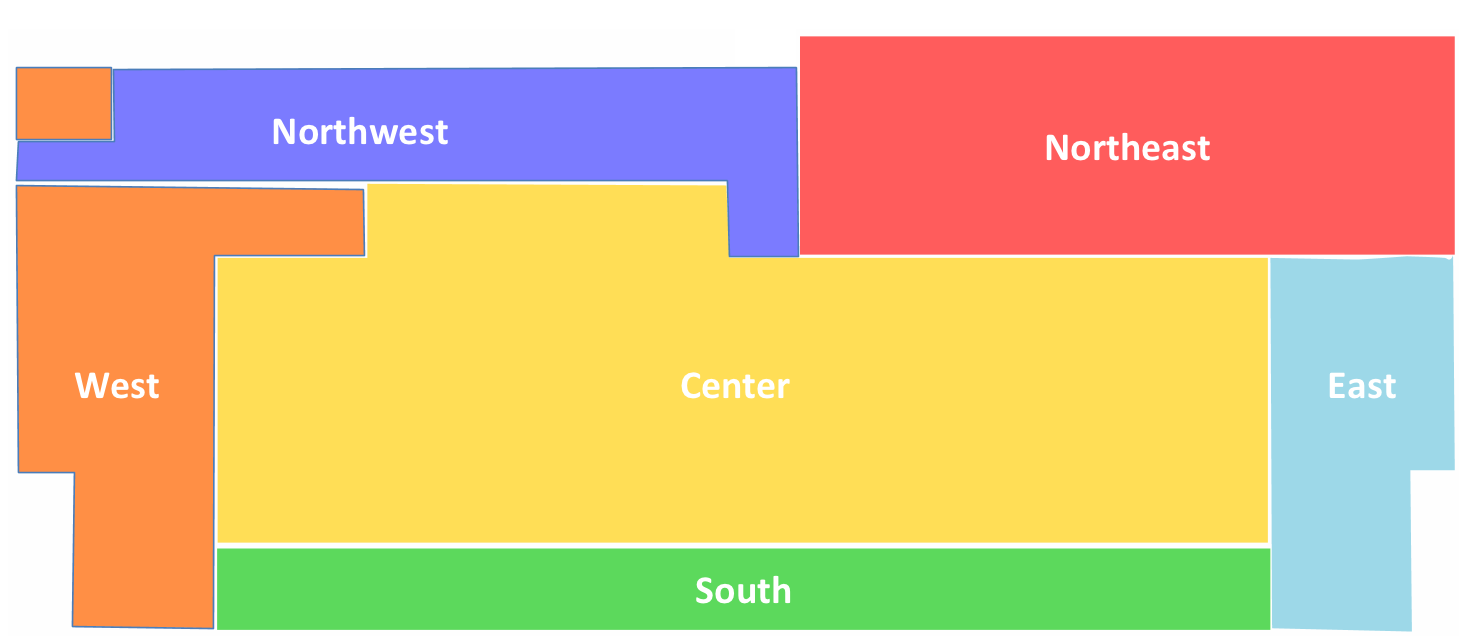
\includegraphics[width=\textwidth]{chapters/building_model/figures/FloorPlan.png}
\vspace*{-0.05cm}
\caption{Zones for the fourth floor of Sutardja Dai Hall (SDH).}
\label{fig:floor_plan}
\vspace*{-0.45cm}
\end{figure}

%\begin{table}[hbtp]
%\centering
%\begin{tabular}{*2c}
%\toprule
%Zone & VAV Boxes \\ \hline
%Northwest (NW) & 6, 8, 11 \\
%West (W) & 1, 2, 3 \\
%South (S) & 5, 9, 15, 16 \\
%East (E) & 20, 21 \\
%Northeast (NE) & 10, 14, 17, 19 \\
%Center (C) & 4, 7, 12, 13, 18 \\
%\bottomrule
%\end{tabular}
%\caption{VAV Boxes by Zone}
%\vspace*{-0.5cm}
%\label{tab:Zone_VAV}
%\end{table}

%%%%%%%%%%%%%%%%%%%%%%%%%%%%%%%%%%%%%%%%%%%%%%%%%%%%%%%%%%

\subsection{Collection of Experimental Data}\label{sec:exp_data}
We collected 36 weeks of one-minute resolution temperature data for the six zones along with the airflow rates of all 21 VAV boxes on the fourth floor, SAT and the outside air temperature from the \textit{simple Measurement and Actuation Profile} (sMAP). sMAP is a protocol that collects, stores and publishes time-series data from a wide variety of sensors \cite{smap, Dawson-Haggerty:2012aa}. The hourly global horizontal solar radiation data was obtained from a nearby weather station \cite{SolarRad}, from which the incidence solar radiation of the four geographic directions was calculated with the \texttt{PV\_LIB} toolbox \cite{pv_model}. All collected data were down-sampled or interpolated, respectively, to 15 minute intervals. 
These 36 weeks of data span periods when the building was under normal operation as well as periods with excitation experiments. 

To increase identifiability of the building model, forced response experiments were performed. These experiments were conducted during Saturdays to (a) minimize effects due to occupancy on our collected data, and thus facilitate subsequent parameter identification; (b) minimize impact to building operation and exploit larger comfort bounds on room temperatures during the weekends. Indeed, the comfort bounds were never violated during the forced experiments. 
%Details on the design of our excitation experiments can be found in \cite{Qie}.
%For accurate parameter identification, temperatures of neighboring zones should not be strongly correlated \cite{Lin_multizone}. 
%For buildings in regular operation, this is generally achievable through forced response experiments. 
Because of commercial buildings' large thermal inertia, each forced excitation must last sufficiently long before temperature changes are observable (we chose 2 hours for our excitation experiment).
More specifically, starting at 8 a.m., the supply air's flow rate to one zone is set to its maximum value every 2 hours. During this 2 hour period, all of its adjacent zones' airflow rates are set to their minimum values, and each of the remaining zones' airflow rate is set to a random value. 
This procedure is repeated for each of the six zones. 
%This experiment is performed during weekends as (a) it minimizes effects due to building occupancy on our data, and thus the subsequent parameter identification; (b) temporary violation of comfort constraints during the weekend was allowed.

%For accurate parameter identification, temperatures of neighboring zones should not have strong correlation \cite{Lin_multizone}. Our testbed is a regular office building in operation, thus forced response experiments were performed during Saturdays to (a) increase identifiability of the building model; (b) minimize effects due to occupancy on our data, and thus facilitate subsequent parameter identification; (c) minimize disturbance to building operation \cite{Qie}.


\subsection{Data Splitting}
Next, we define the seasons ``fall" (early September until mid December), ``winter" (mid December until late January), and ``spring" (late January until mid May) in order to account for different occupancy levels during the fall and spring semesters, and the winter break. After the weeks have been assigned to the seasons, a random portion of the data in each season (e.g. we chose 90\%) was defined as the training data, and the remaining weeks to be removed prior to the analysis were declared as the test set, which were used to assess the accuracy of the building model fitted on the training data.

%\subsection{Notation}
%\label{sec:Notation}
%Let $\hat{\left( \cdot \right)}$ denote either the conditional expectation or the estimated value of a variable. Let $\tilde{\left( \cdot \right)}$ the predicted value of a variable, respectively.

%\qie{I removed bold face for vectors and matrices, because otherwise every equation for the individual zone model and physics based model will be in bold face. Also for notation consistency, I thought about changing the x and v in the physics-based model to T and w, but since it is a state space model, I think it would be clearer to stick to the standard notation for state space models, where x is the state (temperature in this case) and v is the disturbance, so I changed all temperatures to x, and disturbances to v.}
